% ---- figure comparaison_distances_line_graphes_cellules_k_2x50
%\begin{figure}[htb!] 
%\centering
%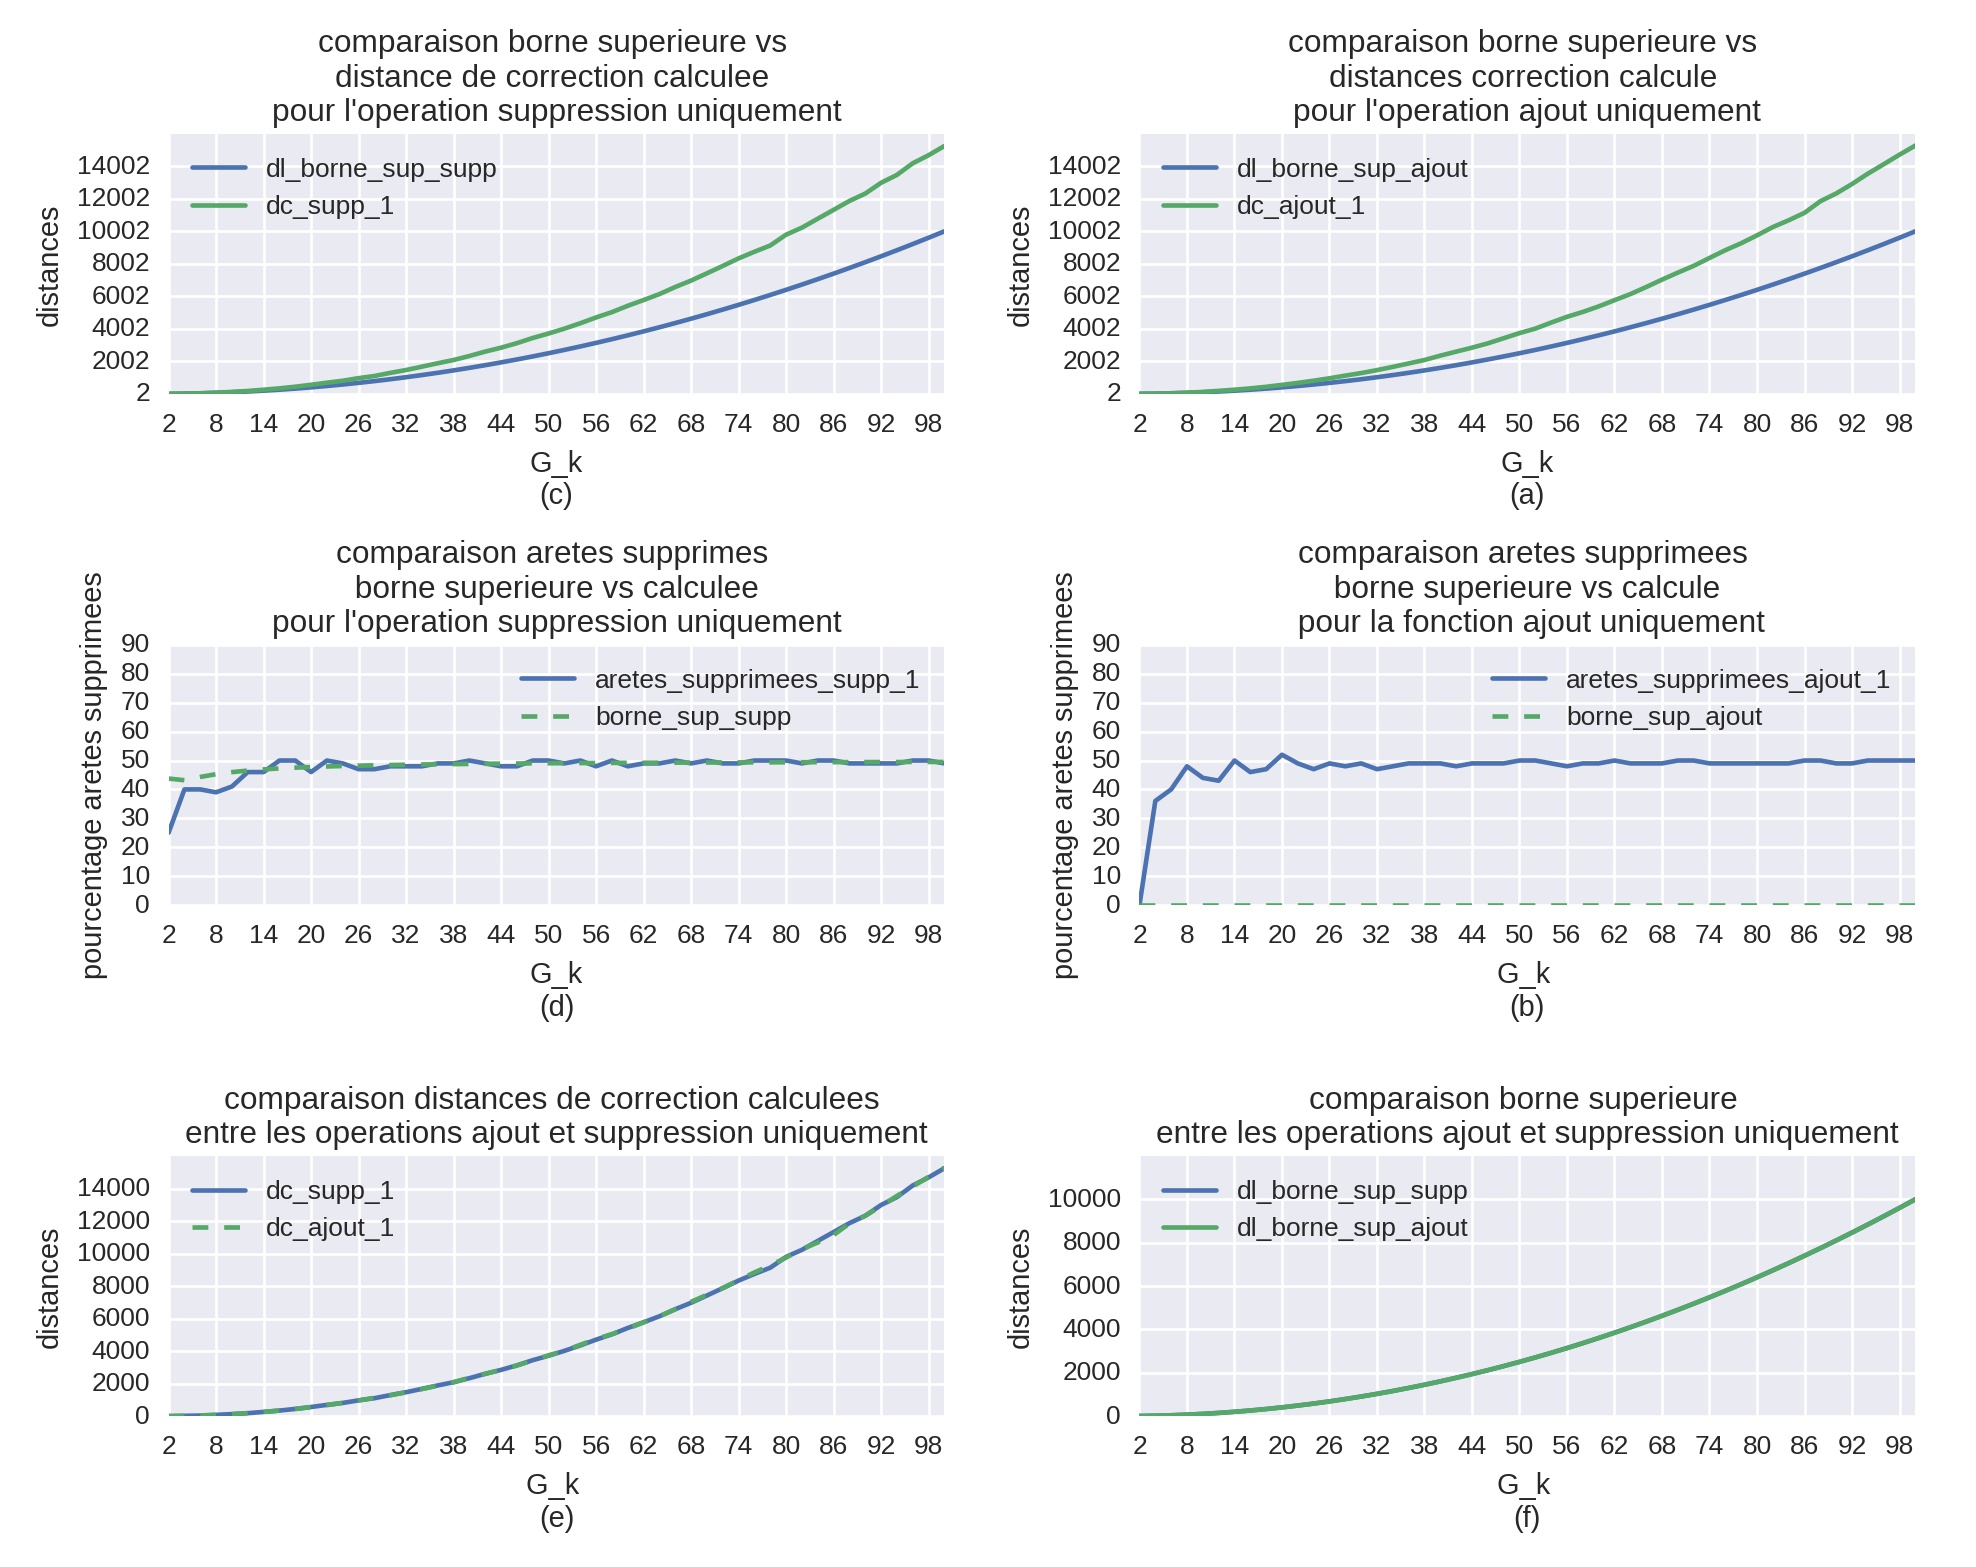
\includegraphics[scale = 0.25]{comparaison_distances_line_graphes_cellules_k_2x50.jpeg}
%\caption{Comparaison de distances lines th\'eoriques et calcul\'ees selon des fonctions de co\^ut {\em suppression} et  {\em ajout}.
%La figure $(a)$ d\'esigne la comparaison entre les distances de correction et la borne sup\'erieure de l'\'equation \ref{borneSuperieureDL} avec la modification {\em ajout d'ar\^etes uniquement}, 
%La figure $(c)$ d\'esigne la comparaison entre les distances de correction et la borne sup\'erieure de l'\'equation \ref{borneSuperieureDL} avec la modification {\em suppression d'ar\^etes uniquement}, 
%La figure $(b)$ compare le pourcentage d'ar\^etes supprim\'ees  dans les graphes boucl\'ees avec celui de la borne sup\'erieure de l'\'equation \ref{borneSuperieureDL} dans la modification {\em ajout d'ar\^etes uniquement}, 
%La figure $(d)$ compare le pourcentage d'ar\^etes supprim\'ees  dans les graphes boucl\'ees avec celui de la borne sup\'erieure de l'\'equation \ref{borneSuperieureDL} dans la modification {\em suppression d'ar\^etes uniquement},
%La figure $(e)$ compare les distances de correction entre les diff\'erentes modifications.
%}
%\label{comparaison_distances_line_graphes_cellules_k_2x50}
%\end{figure}
%\FloatBarrier
\begin{figure}[htb!] 
\centering
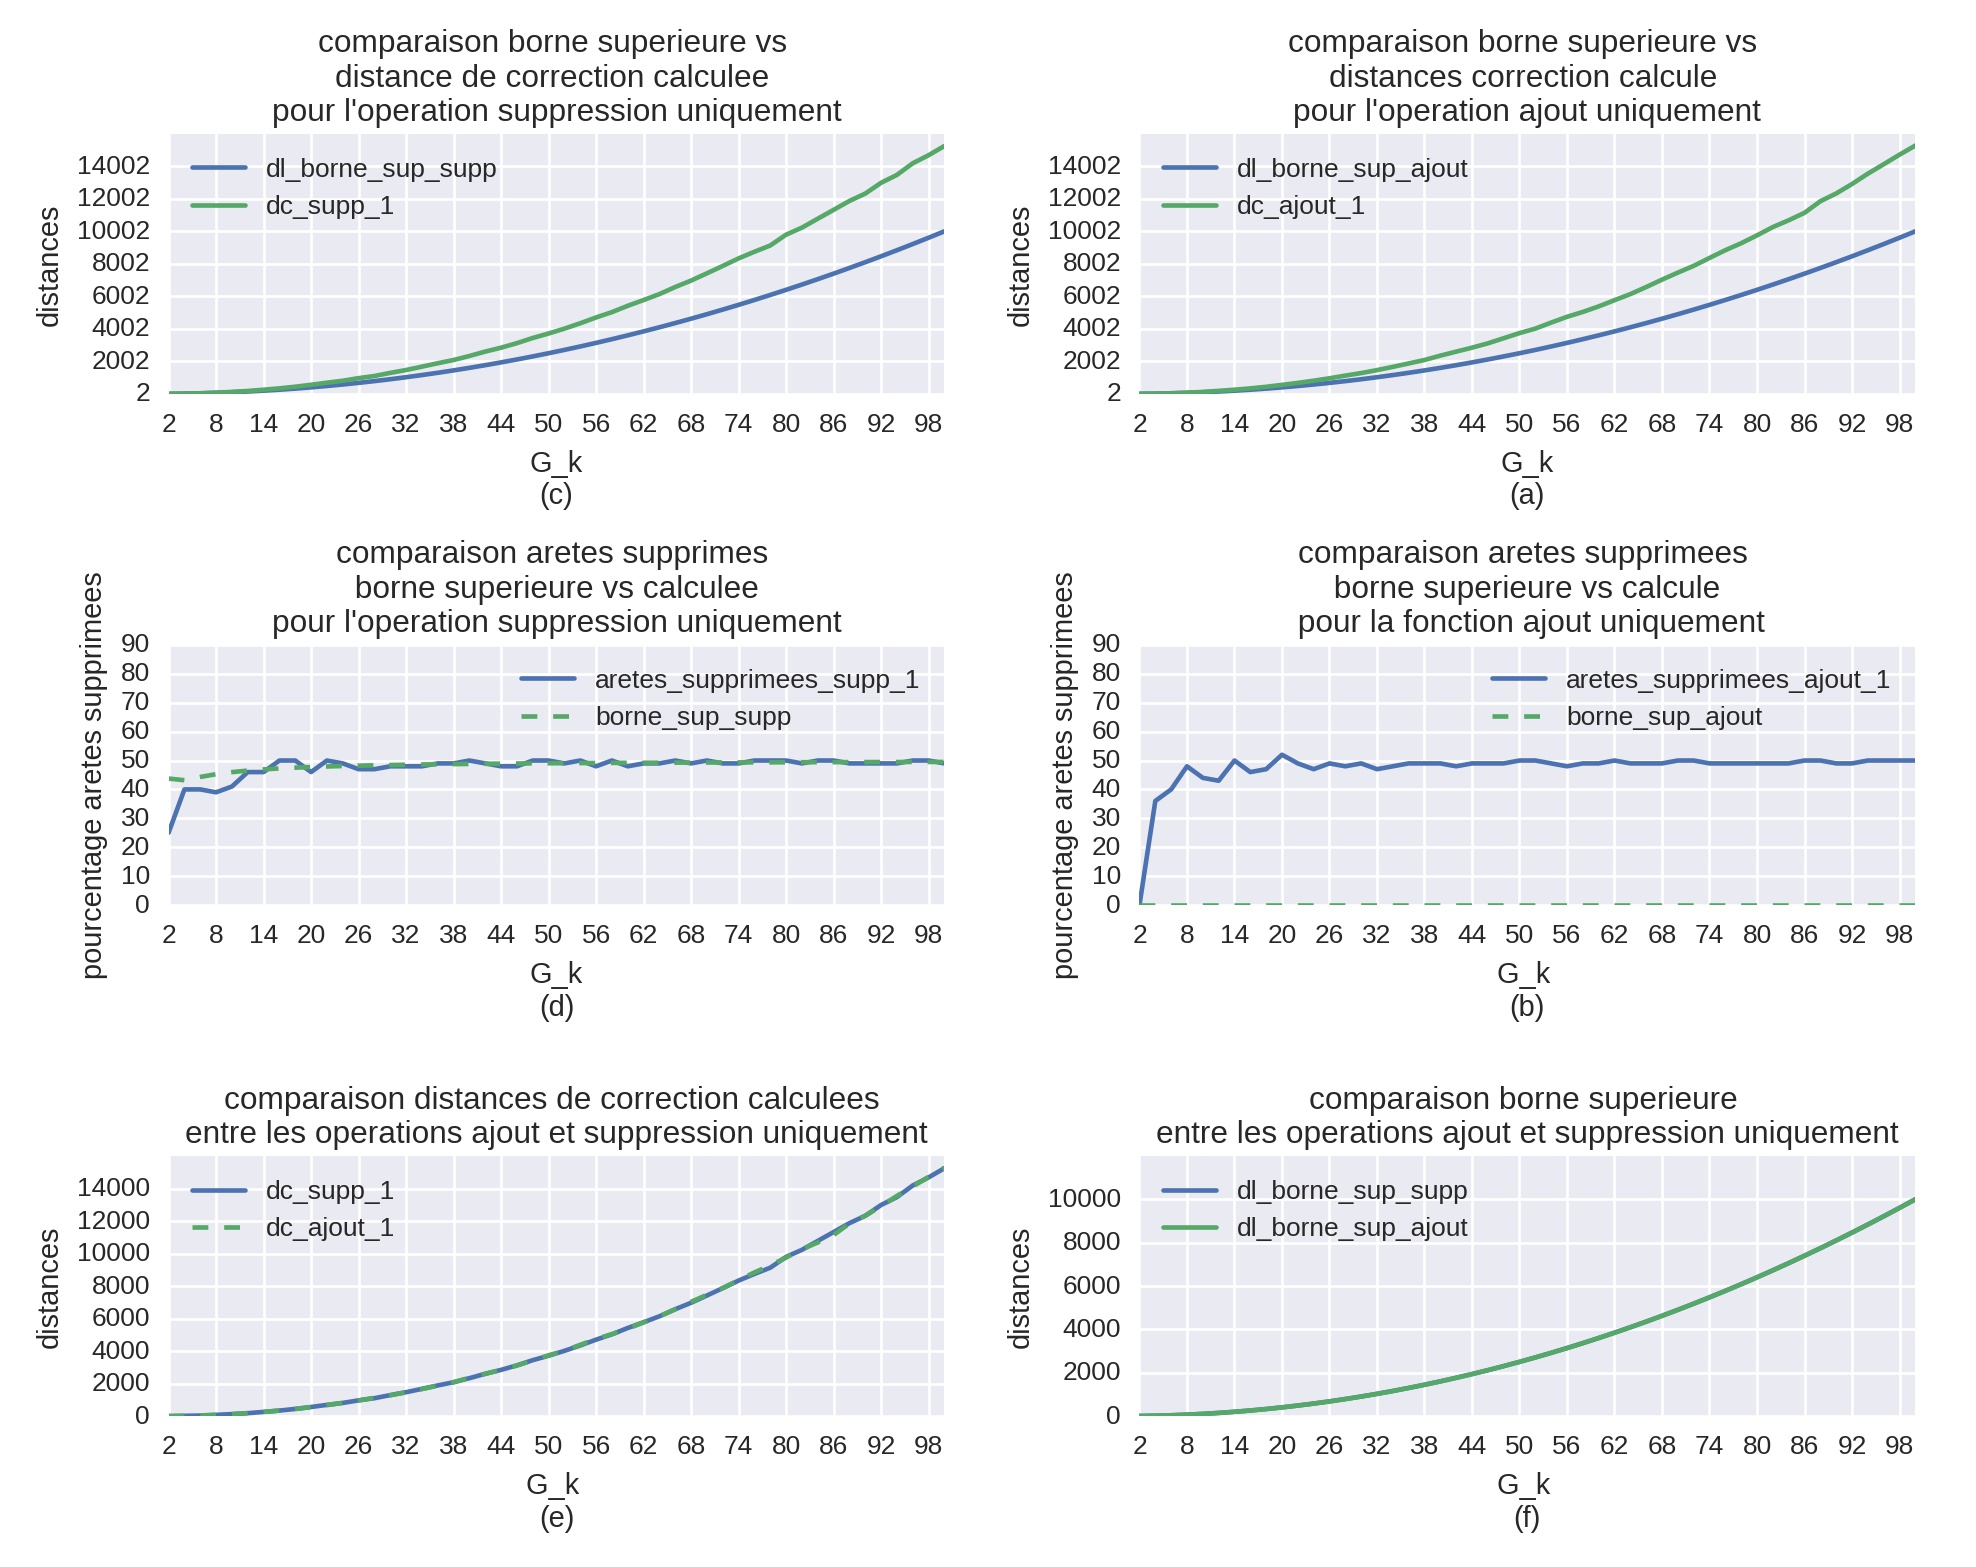
\includegraphics[scale = 0.25]{comparaison_distances_line_graphes_cellules_k_2x50.jpeg}
\caption{Comparaison entre la borne sup\'erieure de la distance line et les distances de correction calcul\'ees selon des fonctions de co\^ut {\em suppression} et  {\em ajout} : 
la figure $(a)$ d\'esigne la comparaison entre les distances de correction et la borne sup\'erieure de l'\'equation \ref{borneSuperieureDL} avec la modification {\em ajout d'ar\^etes uniquement}, 
la figure $(c)$ d\'esigne la comparaison entre les distances de correction et la borne sup\'erieure de l'\'equation \ref{borneSuperieureDL} avec la modification {\em suppression d'ar\^etes uniquement}, 
la figure $(b)$ compare le pourcentage d'ar\^etes supprim\'ees  dans les graphes boucl\'ees avec celui de la borne sup\'erieure de l'\'equation \ref{borneSuperieureDL} dans la modification {\em ajout d'ar\^etes uniquement}, 
la figure $(d)$ compare le pourcentage d'ar\^etes supprim\'ees  dans les graphes boucl\'ees avec celui de la borne sup\'erieure de l'\'equation \ref{borneSuperieureDL} dans la modification {\em suppression d'ar\^etes uniquement},
la figure $(e)$ compare les distances de correction entre les diff\'erentes modifications.
}
\label{comparaison_distances_line_graphes_cellules_k_2x50}
\end{figure}
%\FloatBarrier
% ---- figure comparaison_distances_line_graphes_cellules_k_2x50


Notre objectif est de pr\'esenter les variations des distances de correction par rapport \`a la borne sup\'erieure de la distance line pour chaque modification r\'ealis\'ee sur les graphes pendant l'algorithme de correction. Pour ce faire, nous regroupons notre analyse en $5$ exp\'erimentations.
\newline

Les deux premi\`eres exp\'erimentations comparent les distances de correction avec la borne sup\'erieure pour la modification {\em ajout d'ar\^etes uniquement} (figure \ref{comparaison_distances_line_graphes_cellules_k_2x50} (a) et 
pour la modification {\em suppression d'ar\^etes uniquement} figure \ref{comparaison_distances_line_graphes_cellules_k_2x50} (c).
Nous constatons que les courbes des distances de correction et celle de la borne sup\'erieure sont croissantes. 
La courbe de la borne sup\'erieure, d\'esign\'ee par $borneSup$ dans les graphiques $(a)$ et $(c)$, \'evolue lentement par rapport aux courbes des distances et l'\'ecart entre ces courbes croit lin\'eairement. 
Pour comprendre cet \'ecart croissant, nous v\'erifions le pourcentage d'ar\^etes  supprim\'ees pour chaque modification.  Ce sont les deux autres exp\'erimentations faites et repr\'esent\'ees par la figure 
\ref{comparaison_distances_line_graphes_cellules_k_2x50} (b) pour la modification {\em ajout d'ar\^etes uniquement} et
 la figure \ref{comparaison_distances_line_graphes_cellules_k_2x50} (d) pour la modification 
{\em suppression d'ar\^etes uniquement}. 
En effet, nous avons choisi les ar\^etes supprim\'ees parce que le nombre d'ar\^etes est d\'ej\`a connu c'est-\`a-dire $0$ pour l'ajout uniquement et la borne sup\'erieure pour la suppression uniquement. 
\newline
Nous remarquons que les ar\^etes   de $G_k$ supprim\'ees avoisinent en moyenne de
$40\%$ quand le nombre $k$ de cellules est petit ($k\le14$) dans la modification {\em ajout ar\^etes uniquement}. Au d\'el\`a de $k > 14$, une ar\^ete sur deux du graphe $G_{k}$ est supprim\'ee. La courbe  $aretes\_supprimees\_ajout\_1$ dans le graphique $(b)$ repr\'esente le pourcentage d'ar\^etes supprim\'ees.  
En effet, nous expliquons ces chiffres  par l'ajout d'ar\^etes entre des sommets de cellules voisines et ces sommets ne sont pas partag\'es entre les cellules voisines. Ces ar\^etes ajout\'ees impliquent la suppression des ar\^etes de $G_k$ parce que la partition $\pi_s$ (voir section \ref{algorithmeCorrection}) des ar\^etes \`a supprimer pendant la compression n'est pas vide et contient des ar\^etes de $G_k$ en g\'en\'eral. Ainsi ces ar\^etes provoquent l'abandon des ar\^etes diagonales  ajout\'ees \`a partir du sommet commun entre des cellules comme indiqu\'e dans l'exemple du graphe $G_{4,4}$ dans la figure \ref{exempleCorrectionGrapheCelluleAvecAjout}.
\newline
En ce qui concerne la modification {\em suppression d'ar\^etes uniquement}, les ar\^etes supprim\'ees proviennent aussi des cellules voisines. 
Dans les cellules partageant un sommet, l'algorithme ajoute g\'en\'eralement une ar\^ete diagonale \`a partir de ce sommet commun dans une seule cellule. Les ar\^etes diagonales ajout\'ees sont responsables de l'augmentation de la distance de correction ( courbe {\em dc\_supp\_1} dans le graphique $(c)$).
Pour des cellules partageant une ar\^ete, l'algorithme supprime certaines ar\^etes communes comme indiqu\'e dans la section \ref{modificationSuppressionAretesUniquement}. Les autres ar\^etes communes non supprim\'ees sont dues \`a la pr\'esence des ar\^etes diagonales. Cela explique pourquoi nous avons en moyenne $50\%$ des ar\^etes de $G_k$ qui sont supprim\'ees dans le graphique $(d)$. Ce pourcentage est identique \`a celui des ar\^etes supprim\'ees de la borne sup\'erieure lorsque le nombre de cellules devient \'elev\'e $k \ge 18$ et il ne signifie pas que l'algorithme de correction supprime les ar\^etes de la section \ref{modificationSuppressionAretesUniquement}.
\newline
Par ailleurs, les courbes {\em dc\_ajout\_1} de la modification d'{\em ajout d'ar\^etes uniquement} et celle {\em dc\_supp\_1}  de la modification {\em suppression d'ar\^etes uniquement} ont les m\^emes tendances et sont superpos\'ees (figure $(e)$) parce que  dans la modification d'{\em ajout}, l'algorithme ajoute la m\^eme proportion d'ar\^etes qu'il supprime dans  la modification {\em suppression}. 
\newline

\vspace{-0.25cm}
{\bf Conclusion} :   
l'exp\'erimentation montre que le line-graphe $L(G_k)$ propos\'e par l'algorithme de correction pour un $k$ donn\'ee est identique en terme de distance de correction quelle que soit la modification r\'ealis\'ee comme illustre la figure \ref{comparaison_distances_line_graphes_cellules_k_2x50}(e).
Toutefois, les graphes corrig\'es ne sont pas optimaux en terme de distances de correction parce que l'algorithme priorise dans certains cas les modifications {\em ajout d'ar\^etes uniquement} et {\em suppression uniquement} et cela leur permet d'atteindre des minimums locaux. Cependant le minimum global n'est pas atteint g\'en\'eralement. 

%Nous r\'ealisons cinq comparaisons et les r\'esultats obtenus sont regroup\'es en $6$ exp\'erimentations.
%\newline
%Les deux premi\`eres exp\'erimentations comparent les distances line th\'eoriques et les distances de correction obtenues apr\`es l'ex\'ecution de nos algorithmes pour chaque op\'eration. Le terme {\em th\'eorique} signifie que le line-graphe obtenu apr\'es la correction du graphe cellule $G_k$ est optimal c'est-\`a-dire la distance line de $G_k$ est minimale. 
%Quant au terme {\em calcul\'e}, il designe les distances obtenues apr\`es l'execution de l'algorithme de correction.
%\newline
%La figure \ref{comparaison_distances_line_graphes_cellules_k_2x50}(c) d\'esigne la comparaison avec l'op\'eration {\em suppression uniquement} entre les bornes sup\'erieures de la distance line th\'eorique {\em dl\_theorique\_supp} et les distances de correction calcul\'ee {\em dc\_supp\_1}. Alors que l'op\'eration {\em ajout uniquement} est repr\'esent\'ee par la figure \ref{comparaison_distances_line_graphes_cellules_k_2x50}(a) dans laquelle nous comparons la borne sup\'erieure des distances line th\'eoriques {\em dl\_theorique\_ajout}  et les distances de correction calcul\'ees {\em dc\_ajout\_1}.  
%
%Les  exp\'erimentations  des figures \ref{comparaison_distances_line_graphes_cellules_k_2x50}$(d)$ et \ref{comparaison_distances_line_graphes_cellules_k_2x50}$(b)$ indiquent, respectivement, le pourcentage d'ar\^etes supprim\'ees dans les grilles $G_k$ pour les op\'erations {\em suppression uniquement} et {\em ajout uniquement}. Nous avons determin\'e th\'eoriquement le nombre d'ar\^etes \`a supprimer pour obtenir le line-graphe optimal et nous comparons ce nombre avec celui des ar\^etes supprim\'ees apr\'es l'ex\'ecution des algorithmes. 
%Les termes {\em aretes\_G\_k\_notIn\_LG\_theoriques\_supp} et {\em aretes\_G\_k\_notIn\_LG\_theoriques\_ajout} d\'esignent, respectivement, la courbe th\'eorique des ar\^etes supprim\'ees dans les grilles $G_k$ pour fournir des line-graphes optimaux avec les op\'erations {\em suppression uniquement} et {\em ajout uniquement}. De m\^eme, les termes {\em aretes\_G\_k\_notIn\_LG\_supp\_1} et  {\em aretes\_G\_k\_notIn\_LG\_ajout\_1} d\'esignent, respectivement, la courbe des ar\^etes supprim\'ees dans les graphes $G_k$ apr\`es l'ex\'ecution des algorithmes pour les op\'erations {\em suppression uniquement} et {\em ajout uniquement}.
%
%La figure \ref{comparaison_distances_line_graphes_cellules_k_2x50}$(e)$ repr\'esente la comparaison entre  les distances de correction qui sont calcul\'ees avec les diff\'erentes op\'erations. Ainsi, {\em dc\_ajout\_1} et {\em dc\_supp\_1} identifient, respectivement, les courbes avec les op\'erations {\em ajout uniquement} et {\em suppression uniquement}. 
%De m\^eme, la figure \ref{comparaison_distances_line_graphes_cellules_k_2x50}$(f)$ compare les bornes sup\'erieures des distances line th\'eoriques avec les diff\'erentes op\'erations. Ainsi, {\em dl\_theorique\_supp} et {\em dl\_theorique\_ajout} identifient, respectivement, les courbes avec les op\'erations {\em suppression uniquement} et {\em ajout uniquement}. 
%\newline
%
%Dans les figures $(a)$ et $(c)$ , nous constatons que les bornes sup\'erieures des distances line th\'eoriques sont inf\'erieures aux distances de correction obtenues apr\`es l'algorithme de correction, peu importe l'op\'eration r\'ealis\'ee.
%L'\'ecart du nombre d'ar\^etes entre les bornes des distances lines th\'eoriques {\em dl\_theorique\_ajout} et les distances de correction calcul\'ees {\em dc\_ajout} dans l'op\'eration {\em ajout uniquement} provient des ar\^etes ajout\'ees entre deux cellules partageant un sommet. Ces ar\^etes sont ajout\'ees entre un sommet de chaque cellule et cela entraine la suppression d'ar\^etes de $G_k$  car la suppression d'ar\^etes lors d'un partitionnement en cliques se r\'ealise sur les ar\^etes de $G_k$. Aussi ces ar\^etes ajout\'ees provoquent l'abandon d'ar\^etes diagonales ajout\'ees \`a partir du sommet commun dans les cellules comme indiqu\'e dans l'exemple du graphe $G_{4,4}$ dans la figure \ref{exempleCorrectionGrapheCelluleAvecAjout}. 
%Les ar\^etes supprim\'ees avoisinent en moyenne $40\%$ quand le nombre de cellules est faible $k\le14$. Au d\'el\`a de $k > 14$, une ar\^ete sur deux du graphe $G_{k}$ est supprim\'ee comme il est indique dans la figure $(b)$.
%La courbe de {\em aretes\_G\_k\_notIn\_LG\_ajout\_1} est nulle parce que nous ne supprimons aucune ar\^ete dans le line-graphe $L(G_k)$ optimal.
%Quant aux cellules ayant une ar\^ete commune, une seule ar\^ete diagonale est ajout\'ee dans chaque cellule \`a partir du m\^eme sommet de l'ar\^ete commune.  
%\newline  
%En ce qui concerne  l'\'ecart entre le nombre d'ar\^etes supprim\'ees th\'eoriques et calcul\'ees, nous pouvons dire que les ar\^etes issues de cet \'ecart proviennent de cellules voisines. Dans les cellules partageant un sommet, l'algorithme ajoute g\'en\'eralement une ar\^ete diagonale \`a partir de ce sommet commun dans une seule cellule. Les ar\^etes diagonales ajout\'es sont responsables de l'augmentation de la distance de correction {\em dc\_supp\_1}.
%Pour des cellules partageant une ar\^ete, l'algorithme supprime l'ar\^ete commune.  Cela explique pourquoi nous avons en moyenne $50\%$ des ar\^etes de $G_k$ qui sont supprim\'ees dans la figure $(d)$ et ce pourcentage est identique avec les ar\^etes supprim\'ees th\'eoriques lorsque le nombre de cellules devient \'elev\'e $k \ge 18$.
%\newline
%Par ailleurs, 
%nous avons en moyenne $2/3$ ar\^etes ajout\'ees et $1/3$ d'ar\^etes supprim\'ees dans les distances line {\em dc\_ajout\_1}. Et dans les distances {\em dc\_supp\_1}, $2/3$ ar\^etes sont des ar\^etes supprim\'ees et $1/3$ sont des ar\^etes ajout\'ees.
%Ceci implique que les courbes des distances   {\em dc\_ajout\_1} et {\em dc\_supp\_1} ont les m\^emes tendances et sont superpos\'ees (figure $(e)$). 
%La superposition des distances line th\'eoriques des diff\'erentes op\'erations (figure $(f)$) est due \`a l'ordre de l'expression litt\'erale de leurs distances. En effet, le d\^egre de polyn\^omes des op\'erations {\em ajout uniquement} et {\em suppression uniquement} est $2$ et les coefficents de ces polyn\^omes sont tr\`es proches. Cette figure nous permet d'affirmer que les op\'erations {\em ajout uniquement} et {\em suppression uniquement} ont les memes bornes sup\'erieures.
%\newline
%
%L'exp\'erimentation montre que les line-graphes $L(G_k)$ propos\'es par l'algorithme de correction sont identiques  en terme de distance de correlction quelle que soit l'op\'eration de correction. Toutefois, les solutions propos\'ees ne sont pas optimales parce que l'algorithme supprime des ar\^etes pendant l'op\'eration {\em ajout uniquement} et ajoute des ar\^etes pendant l'operation {\em suppr\'ession uniquement}.  
